% Options for packages loaded elsewhere
\PassOptionsToPackage{unicode}{hyperref}
\PassOptionsToPackage{hyphens}{url}
%
\documentclass[
  man,floatsintext]{apa6}
\usepackage{amsmath,amssymb}
\usepackage{iftex}
\ifPDFTeX
  \usepackage[T1]{fontenc}
  \usepackage[utf8]{inputenc}
  \usepackage{textcomp} % provide euro and other symbols
\else % if luatex or xetex
  \usepackage{unicode-math} % this also loads fontspec
  \defaultfontfeatures{Scale=MatchLowercase}
  \defaultfontfeatures[\rmfamily]{Ligatures=TeX,Scale=1}
\fi
\usepackage{lmodern}
\ifPDFTeX\else
  % xetex/luatex font selection
\fi
% Use upquote if available, for straight quotes in verbatim environments
\IfFileExists{upquote.sty}{\usepackage{upquote}}{}
\IfFileExists{microtype.sty}{% use microtype if available
  \usepackage[]{microtype}
  \UseMicrotypeSet[protrusion]{basicmath} % disable protrusion for tt fonts
}{}
\makeatletter
\@ifundefined{KOMAClassName}{% if non-KOMA class
  \IfFileExists{parskip.sty}{%
    \usepackage{parskip}
  }{% else
    \setlength{\parindent}{0pt}
    \setlength{\parskip}{6pt plus 2pt minus 1pt}}
}{% if KOMA class
  \KOMAoptions{parskip=half}}
\makeatother
\usepackage{xcolor}
\usepackage{graphicx}
\makeatletter
\def\maxwidth{\ifdim\Gin@nat@width>\linewidth\linewidth\else\Gin@nat@width\fi}
\def\maxheight{\ifdim\Gin@nat@height>\textheight\textheight\else\Gin@nat@height\fi}
\makeatother
% Scale images if necessary, so that they will not overflow the page
% margins by default, and it is still possible to overwrite the defaults
% using explicit options in \includegraphics[width, height, ...]{}
\setkeys{Gin}{width=\maxwidth,height=\maxheight,keepaspectratio}
% Set default figure placement to htbp
\makeatletter
\def\fps@figure{htbp}
\makeatother
\setlength{\emergencystretch}{3em} % prevent overfull lines
\providecommand{\tightlist}{%
  \setlength{\itemsep}{0pt}\setlength{\parskip}{0pt}}
\setcounter{secnumdepth}{-\maxdimen} % remove section numbering
% Make \paragraph and \subparagraph free-standing
\ifx\paragraph\undefined\else
  \let\oldparagraph\paragraph
  \renewcommand{\paragraph}[1]{\oldparagraph{#1}\mbox{}}
\fi
\ifx\subparagraph\undefined\else
  \let\oldsubparagraph\subparagraph
  \renewcommand{\subparagraph}[1]{\oldsubparagraph{#1}\mbox{}}
\fi
\ifLuaTeX
\usepackage[bidi=basic]{babel}
\else
\usepackage[bidi=default]{babel}
\fi
\babelprovide[main,import]{english}
% get rid of language-specific shorthands (see #6817):
\let\LanguageShortHands\languageshorthands
\def\languageshorthands#1{}
% Manuscript styling
\usepackage{upgreek}
\captionsetup{font=singlespacing,justification=justified}

% Table formatting
\usepackage{longtable}
\usepackage{lscape}
% \usepackage[counterclockwise]{rotating}   % Landscape page setup for large tables
\usepackage{multirow}		% Table styling
\usepackage{tabularx}		% Control Column width
\usepackage[flushleft]{threeparttable}	% Allows for three part tables with a specified notes section
\usepackage{threeparttablex}            % Lets threeparttable work with longtable

% Create new environments so endfloat can handle them
% \newenvironment{ltable}
%   {\begin{landscape}\centering\begin{threeparttable}}
%   {\end{threeparttable}\end{landscape}}
\newenvironment{lltable}{\begin{landscape}\centering\begin{ThreePartTable}}{\end{ThreePartTable}\end{landscape}}

% Enables adjusting longtable caption width to table width
% Solution found at http://golatex.de/longtable-mit-caption-so-breit-wie-die-tabelle-t15767.html
\makeatletter
\newcommand\LastLTentrywidth{1em}
\newlength\longtablewidth
\setlength{\longtablewidth}{1in}
\newcommand{\getlongtablewidth}{\begingroup \ifcsname LT@\roman{LT@tables}\endcsname \global\longtablewidth=0pt \renewcommand{\LT@entry}[2]{\global\advance\longtablewidth by ##2\relax\gdef\LastLTentrywidth{##2}}\@nameuse{LT@\roman{LT@tables}} \fi \endgroup}

% \setlength{\parindent}{0.5in}
% \setlength{\parskip}{0pt plus 0pt minus 0pt}

% Overwrite redefinition of paragraph and subparagraph by the default LaTeX template
% See https://github.com/crsh/papaja/issues/292
\makeatletter
\renewcommand{\paragraph}{\@startsection{paragraph}{4}{\parindent}%
  {0\baselineskip \@plus 0.2ex \@minus 0.2ex}%
  {-1em}%
  {\normalfont\normalsize\bfseries\itshape\typesectitle}}

\renewcommand{\subparagraph}[1]{\@startsection{subparagraph}{5}{1em}%
  {0\baselineskip \@plus 0.2ex \@minus 0.2ex}%
  {-\z@\relax}%
  {\normalfont\normalsize\itshape\hspace{\parindent}{#1}\textit{\addperi}}{\relax}}
\makeatother

\makeatletter
\usepackage{etoolbox}
\patchcmd{\maketitle}
  {\section{\normalfont\normalsize\abstractname}}
  {\section*{\normalfont\normalsize\abstractname}}
  {}{\typeout{Failed to patch abstract.}}
\patchcmd{\maketitle}
  {\section{\protect\normalfont{\@title}}}
  {\section*{\protect\normalfont{\@title}}}
  {}{\typeout{Failed to patch title.}}
\makeatother

\usepackage{xpatch}
\makeatletter
\xapptocmd\appendix
  {\xapptocmd\section
    {\addcontentsline{toc}{section}{\appendixname\ifoneappendix\else~\theappendix\fi\\: #1}}
    {}{\InnerPatchFailed}%
  }
{}{\PatchFailed}
\keywords{Gender difference, Advice, Interpresonal relationship\newline\indent Word count: 4,362}
\usepackage{csquotes}
\usepackage{setspace, appendix, placeins, booktabs, tikz, siunitx}
\usepackage{tabularx, epigraph, float, colortbl, tabu, pdflscape}
\usetikzlibrary{positioning}
\raggedbottom
\usepackage[maxfloats=256]{morefloats}
\maxdeadcycles=1000
\ifLuaTeX
  \usepackage{selnolig}  % disable illegal ligatures
\fi
\IfFileExists{bookmark.sty}{\usepackage{bookmark}}{\usepackage{hyperref}}
\IfFileExists{xurl.sty}{\usepackage{xurl}}{} % add URL line breaks if available
\urlstyle{same}
\hypersetup{
  pdftitle={Interpersonal Benefits of Flattering Advice},
  pdfauthor={Amanda Chen1 \& David Hagmann1},
  pdflang={en-EN},
  pdfkeywords={Gender difference, Advice, Interpresonal relationship},
  hidelinks,
  pdfcreator={LaTeX via pandoc}}

\title{Interpersonal Benefits of Flattering Advice}
\author{Amanda Chen\textsuperscript{1} \& David Hagmann\textsuperscript{1}}
\date{}


\shorttitle{Flattering Advice}

\authornote{

The authors are grateful to a lot of things.

Correspondence concerning this article should be addressed to Amanda Chen, Department of Management, The Hong Kong University of Science and Technology, Hong Kong. E-mail: \href{mailto:zchengj@connect.ust.hk}{\nolinkurl{zchengj@connect.ust.hk}}

}

\affiliation{\vspace{0.5cm}\textsuperscript{1} The Hong Kong University of Science and Technology}

\note{

1 January, 2024

}

\abstract{%
This is an interesting project! Please read through it!
}



\begin{document}
\maketitle

\hypertarget{introduction}{%
\section{Introduction}\label{introduction}}

Gender differences have been documented in various domains and attract plenty of scholarly attention to explain underlying causes. Extent research largely focuses on internal factors, such as cognitive styles, preference, personal beliefs, assuming females and males want to do different things. Another source of such differences may be the advice that people receive. Prior work has documented that men receive more aspirational advice and women more risk-averse advice, which may explain why women are less likely to apply for and ultimately obtain more rewarding positions. Research in this line of gender discrimination has emphasized the role of unconscious bias, but interventions that try to reduce this bias have been largely unsuccessful.
This paper propose a novel source of differences in advice by drawing on recent work on belief-based utility, expectation-based reference points, and the hedonic consequences of information. Specifically, we hypothesize that receiving information that is less favorable than one expects imposes a psychological cost on the recipient, because it is disappointing and suggests a less favorable future than one imagined. If people anticipate this cost when giving advice, they may be overly favorable or optimistic so as to protect the advisee's belief utility. That is, they may not (only) give the advice that they believe will lead to the best decision but are also motivated to avoid disappointing the recipient. This requires the formation of beliefs about the advisee's expectations, which is where we propose the differential treatment of men and women arises. Prior work has documented that men are more overconfident than women, conditional on equal performance, and that people anticipate this difference. An adviser who seeks to avoid disappointment and incorporates expectations into their advice would then present more favorable advice to male advisees than to female advisees.
While the interpersonal concern has not been fully investigated as a source of gender difference regarding advice giving, its assumption, the hedonic consequences of information have been well documented. Research in economics and psychology has found that people avoid information that could make them feel bad, even when doing so leads to worse decisions. Recipients of information are even found to blame the people who deliver undesirable message, even though the messenger are not responsible for the situation.
Advice is predicted to trigger a more intense emotional response because it is assumed to be tailored for its target, and reflects how the giver see the target. Individuals tend to desire positive social images and are protective when it comes to others' evaluation of them, and accordingly, prefer advice that implies a positive evaluation. However, we are unaware of research documenting whether people take this into account when advising others.

\hypertarget{a.-our-study}{%
\section{A. Our study}\label{a.-our-study}}

We test whether gender difference in receiving advice is driven by givers' intention to meet target's expectation and avoid disappoint them. We report results from two preregistered experiment in which the interactions without deception between advice givers and recipients are captured. In each experiment, we first measure actual level and expectations of advisees, then provide these information to givers and collect advice. Lastly, we present advice to their targets, ask advisees to make final decision, and measure the utility of the advice.
We predict and find that males receive flattering advice than female counterparts when advisers take target's expectations into account. If advice for both gender is solely based on actual performance, there exists no gender difference regarding the chance of receiving aggressive advice. But when expectation of the target is provided along with actual performance, advisers consider this irrelevant information and give more aggressive advice to males because they have higher expectations for themselves compared with equally competent females.
We also directly test the reason why advisers provide flattering advice. We compare advice given under the treatment condition where interpersonal concerns is the goal with that of baseline condition where, like usually assumed, effectiveness of facilitating decision making is emphasized. Advisers are more likely to inflate their advice so that it delivers a positive evaluation of its target when they hold interpersonal concerns and want to be liked by the target.

\hypertarget{b.-related-literature}{%
\section{B. Related Literature}\label{b.-related-literature}}

People frequently obtain information by soliciting the advice of those with more expertise about or insight into an issue. A substantial literature has studied how people incorporate advice and whose advice they seek out. Briefly, people put less than optimal weight on the advice they receive, and prefer advice from those who are overconfident or who provide favorable information. Indeed, people punish advisers who tell them things they do not want to hear. Most of the studies in this stream of research have relied on deception and do not involve real people in the role of advisers; studies of advisers themselves remain scarce.

Notably, prior work on advice has emphasized the instrumental value of information, examining the extent to which the advice improves the quality of or satisfaction with a decision. In the proposed project, we will focus on the signaling value of advice: what does the advice imply about the adviser's perception of the advisee? We propose that ``flattering'' advice creates a perception that the adviser holds the advisee in high esteem, and that this in turn increases the advisee's liking for the adviser. Such interpersonal considerations may be as important (or even more important) in cases where it is difficult to evaluate ex post whether the advice was good or not.

Prior work has further documented that men and women receive different performance feedback at work. Managers are less likely to provide critical feedback to women, believing that doing so would hurt their feelings. Thus, interpersonal concerns can undermine constructive feedback, which then harms outcomes because it deprives the advisee of a learning opportunity. While this effect at first glance appears counter to our hypotheses (here, men receive more negative feedback), it is driven by different beliefs. Managers withhold critical feedback because they (perhaps incorrectly) believe that women suffer a greater cost from criticism. Our hypothesized effect is driven by (accurate) beliefs about performance expectations. While advice also communicates beliefs about ability, it does not do so through criticism.

\hypertarget{study-1}{%
\section{Study 1}\label{study-1}}

In this study, we conducted an initial test to examine whether individuals take others' self-expectations into account when giving advice. Specifically, we predicted that people would adjust their advice to match the advisees' expectations of themselves, even when these expectations are not informative for the underlying decision problem. This study was preregistered on AsPredicted (\url{https://aspredicted.org/R44_6SR}).

\hypertarget{methods}{%
\subsection{Methods}\label{methods}}

We recruited 1,002 participants (50\% Female, \(M_{\text{Age}}\) = 42.13) from Prolific Academic to take math test and another 1,000 (50\% Female, \(M_{\text{Age}}\) = 38.79)
This study consisted of three stages involving recipients of advice taking an exam in Stage 1, givers providing advice in Stage 2, and recipients reacting to advice in Stage 3. During Stage 1, participants were asked to answer ten math questions in five minutes and were informed that they would receive 10 cents for each question they answered correctly. Participants were also asked to predict how many questions they would answer correctly. We manipulated their self-expectations by randomly assigning participants to either a High or Low Expectation condition. In the High Expectation condition, participants were informed that the average score of five other participants who took the same test was 6.4, while those in the Low Expectation condition were told that the average score was 2.6. We incentivized their performance in the math test to increase their attachment to the task. The number of correct answers and their predictions represented the recipients' performance and expectations, respectively, and were shown to advice givers.
After collecting performance and expectations from recipients, we recruited 1,000 participants and informed them of the results of the mathematics quiz completed by the first group of participants. Their task was to give advice to the previous participants about whether to compete against a group of ``high'' performers or a group of ``low'' performers (the top 20 and bottom 20 performers out of a separate group of 50 participants who completed the mathematics quiz). Advisees could earn a bonus if they performed as well or better than a randomly selected member of their chosen group, and the bonus differed depending on the group they chose (50 cents and 30 cents for the high-performing and low-performing group, respectively). Advisers received a bonus identical to the one earned by one of their advisees. They provided advice to 10 randomly selected advisees, and we clustered standard errors at the level of Stage 2 participants in subsequent analyses accordingly. We randomly assigned advisers to one of two conditions: they either observed only the true performance of the advisee (``Baseline'' treatment), or they observed the true performance and the participant's own estimate of their performance (``Information'' treatment). To give givers some sense of this task, we told them the average scores for a previous batch of 50 quiz-takers were 4.42. It is important to note that the advisee's own guess provided no information about the likelihood of winning against either the high or low group, as the outcome was based on past performance and not performance on a subsequent test.
Lastly, we invited the recipients back, reminded them of their previous self-expectations, and informed them that they could earn a bonus if they performed as well or better than a competitor. They could decide where that competitor was randomly drawn from, a group of ``high'' performers or a group of ``low'' performers. If they scored the same or higher than that competitor, they could earn a bonus, whose value differed depending on the group they chose (50 cents and 30 cents for the high-performing and low-performing group, respectively). Recipients were told that an external observer had provided a piece of advice. They then read the advice and made their decisions about who they wanted to compete with.

\hypertarget{open-science-statement}{%
\subsection{Open Science Statement}\label{open-science-statement}}

We report all manipulations, measures, and data exclusion in this and the following study.
The preregistration reports, screenshots of all experimental materials, and
the analysis code to replicate all statistical analyses and figures are
available on the Open Science Framework (will do this later).

\hypertarget{results}{%
\subsection{Results}\label{results}}

We begin by analyzing the performance and expectations of Stage 1 participants, as they will serve as input for Stage 2 participants and influence their advice. We compare the performance and expectations of participants in High and Low Expectation conditions, where they are told the average score for a five-participant group is 6.4 or 2.6. Although we randomly assigned participants, those in the Low Expectation condition scored slightly higher than those in the High Expectation condition (4.80 and 4.55, respectively, \(t(1000) = -1.67\), \(p = .095\)). However, the gap is not significant. Participants in the High Expectation condition had worse performance, but they also indicated a significantly higher guess of their score than their counterparts in the other condition (4.80 and 4.42, respectively, \(t(1000) = 3.72\), \(p < .001\)).It makes our experiment a conservative test. The gap between their expectations is 0.52, which is not marginal considering the average expectations for all participants is only 4.16.It is worth mentioning that participants from both conditions reported having a hard time answering the math test, and thus, they are underconfident. However, participants from the High Expectation condition expected to solve more, indicating a successful manipulation. Despite the manipulation, the expectations are significantly correlated with the actual performance (\(b = 0.63\), 95\% CI \([0.58, 0.67]\), \(t(999) = 27.06\), \(p < .001\)).
Next, we examine gender differences and find that male participants performed slightly better than female participants, and the gap is significant (5.02 and 4.33, respectively, \(t(1000) = -4.77\), \(p < .001\)). On average, males are more confident than females, as they predicted to answer more questions correctly (4.75 and 3.56, respectively, \(t(1000) = -8.65\), \(p < .001\)). We conducted an OLS regression with the performance and gender of participants and found that with the same score, male participants are more confident than their female counterparts (\(b = 0.78\), 95\% CI \([0.56, 0.99]\), \(t(999) = 7.18\), \(p < .001\)).

\begin{table}

\caption{\label{tab:study1regs}Advice of competing against High Performance group, based on the gender of targets and whether their expectation is shown to adviser (Column 1). Column 2 show the results where standard errors are clusterd at the level of adviser. Expeccted Bonus of advice received, based on the gender of targets and whether their expectation is shown to adviser (Column 3)}
\centering
\resizebox{\linewidth}{!}{
\begin{tabular}[t]{lccc}
\toprule
  & (1) & (2) & (3)\\
\midrule
Expectation Shown & \num{-0.034}** & \num{-0.034}* & \num{0.000}\\
 & (\num{0.013}) & (\num{0.013}) & (\num{0.003})\\
Advisee Male & \num{0.002} & \num{0.002} & \num{0.000}\\
 & (\num{0.013}) & (\num{0.005}) & (\num{0.001})\\
Expectation x Male & \num{0.032}+ & \num{0.032}*** & \num{-0.005}**\\
 & (\num{0.019}) & (\num{0.009}) & (\num{0.002})\\
Constant & \num{0.339}*** & \num{0.339}*** & \num{0.258}***\\
 & (\num{0.009}) & (\num{0.010}) & (\num{0.002})\\
\midrule
N & \num{10000} & \num{10000} & \num{10000}\\
\bottomrule
\multicolumn{4}{l}{\rule{0pt}{1em}+ p $<$ 0.1, * p $<$ 0.05, ** p $<$ 0.01, *** p $<$ 0.001}\\
\end{tabular}}
\end{table}

\begin{figure}

{\centering 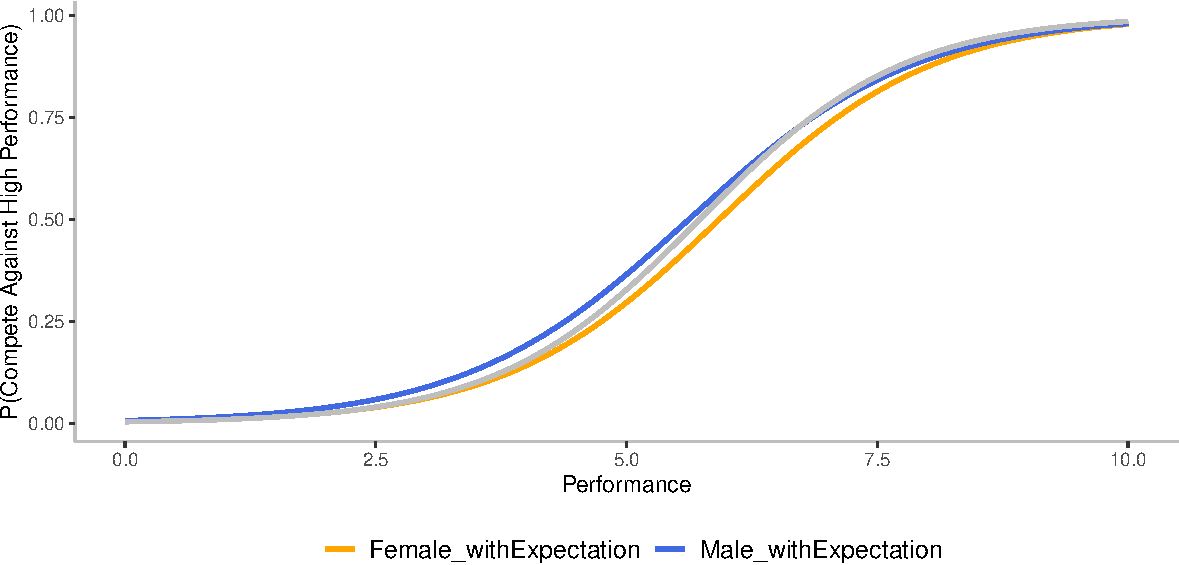
\includegraphics{Advice-Giving_files/figure-latex/study1gender-1} 

}

\caption{When expectation is shown to the adviser}\label{fig:study1gender}
\end{figure}

In Stage 2, we collected 10,000 pieces of advice for 888 Advisees. To exclude between-person differences from advice givers, we clustered standard errors at the level of the Stage 2 participants when running OLS regression. We conducted an OLS regression with the performance and Advisee Treatment (High or Low Expectation) for the subset of Stage 2 participants in the ``Information'' Treatment. Although Advisees in the High Expectation condition are more likely to be recommended to compete against the High Performer Group, the result is not significant (\(b = -0.01\), 95\% CI \([-0.03, 0.01]\), \(t(4997) = -1.13\), \(p = .257\)). This may be because the confidence difference (0.60) is too minor for advice givers to take more risk. Only 33.11\% of the time, advice givers recommended the High Performer group as the competitor, and the average scores for those who received this advice is 6.64, which is about at the 80th percentile in the performance distribution shown to the advice givers.
However, if we run an OLS regression with performance and the exact expectations of Advisees, the expectation does increase the chance of receiving aggressive advice (\(b = 0.03\), 95\% CI \([0.02, 0.04]\), \(t(4997) = 10.13\), \(p < .001\)).
In Stage 2, each participant always sees five females and five males with the same score distribution, and the only difference lies in their expectations. Therefore, we predict that there will be no gender difference when advice givers only see performance, but males will receive more aggressive advice when their expectations are presented. We conducted an OLS regression with whether givers see the expectation (Baseline or Information condition) and the gender of the Advisee (Female or Male), as well as their interaction. In line with our prediction, only when expectations are known to the advice giver, male participants have a higher chance of being recommended to compete against the High Performer group (Column 2 of Table \ref{tab:study1regs} ). As seen in Figure \ref{fig:study1gender}, gender differences emerge as a result of showing expectations.
Because we only have advice for 888 Advisees, to ensure that every participant in Stage 1 receives advice, we recruited 48 more participants to collect more advice for the other 112 participants for Stage 1. We did not include any of this advice in the analysis of Stage 2 results.

Among 1,002 participants, 94.91\% of them returned for the Stage 3 experiment. Of all advice shown to Advisees, 483 of them are from givers in the `Information' treatment condition, and the other 468 are from givers in the `Baseline' treatment condition. To examine the impact of flattering advice on performance, we first looked at advice from givers who know the expectations of Advisees. We conducted an OLS regression with performance and Treatment condition (High or Low Expectation) of Advisees. As predicted, participants in the High Expectation condition received less (\(b = -0.02\), 95\% CI \([-0.05, 0.00]\), \(t(480) = -1.61\), \(p = .107\)), but it is not significant. We realize this result is less powerful because the advice presented was randomly selected and advisees who return to this follow-up survey also bring noise.
To avoid randomness, we computed the Expected Bonus for all 10,000 advice we collected in Stage 2, assuming they are adopted by the Advisees. We conducted an OLS regression with whether givers see the expectation (Baseline or Information condition) and the gender of the Advisee (Female or Male), as well as their interaction. Supporting our theory, male participants will receive less bonus given advice they receive (Column 3 of Table \ref{tab:study1regs} ). It implies that when males receive more aggressive advice (competing against the High Performer group), they end up worse because this kind of advice is not necessarily based on their actual condition.

\hypertarget{study-2}{%
\section{Study 2}\label{study-2}}

In the previous study, we found that individuals take into account the self-expectations of others when providing advice. In this study, we aimed to investigate whether people inflate advice due to the concern for interpersonal benefits. We hypothesized that individuals may exaggerate their advice in order to be viewed more favorably by the recipients. This study was preregistered on AsPredicted (\url{https://aspredicted.org/45P_93G}).

\hypertarget{method}{%
\subsection{Method}\label{method}}

We recruited 207 workers from Prolific (52\% Female, \(M_{\text{Age}}\) = 39.50) to upload selfies and another 472 (50\% Female, \(M_{\text{Age}}\) = 41.03) participants to rate selfies regarding physical attractiveness and give advice.
Study 2 consists of three surveys. At time 1, we invited participants to upload photos of themselves (selfies) to be rated by other participants on attractiveness. We assigned each participant to a group of 10 participants of their own gender. We also asked participants to predict how they rank in this 10-person group regarding physical attractiveness. To create a gender-balanced sample, among all 107 female participants who uploaded selfies, we select the first 100 and only include them in the following time 2 and time 3 studies. That is, in total we have 200 recipients. Next, we recruited 472 new participants and asked them to rank the attractiveness of one such group of 10 participants of the opposite gender. After they did so, we showed them the photo of the participant they ranked as the 7th most attractive (that is, the 4th least attractive) and reminded them that they had ranked this person at 7th place. We (truthfully) informed them that this participant would have a chance to earn a bonus if they accurately guessed their rank based on the aggregated ratings of all participants who had ranked this group. Participants were then randomly assigned to an ``accuracy'' or a ``likability'' treatment. In the accuracy treatment, they received a bonus identical to that of the advisee. In the ``likability'' treatment, their bonus depended on how the advisee rated them in terms of likability, after observing only the rank that they had advised the advisee to guess. At time 3, we invited the participants who uploaded selfies to return for the third stage of the experiment. Here, they observed the rank proposed by an adviser and made an incentivized bet on how they ranked across all of those who rated their photo. We then asked participants to evaluate the adviser based on their likability and warmth on a 5-point scale. The latter dimension was measured with 4-item scale adopted from Fiske, Cuddy, and Glick (2007).

\hypertarget{open-science-statement-1}{%
\subsection{Open Science Statement}\label{open-science-statement-1}}

We report all manipulations, measures, and data exclusion in this and the following study.
The preregistration reports, screenshots of all experimental materials, and
the analysis code to replicate all statistical analyses and figures are
available on the Open Science Framework (will do this later).

\hypertarget{results-1}{%
\subsection{Results}\label{results-1}}

\begin{figure}

{\centering 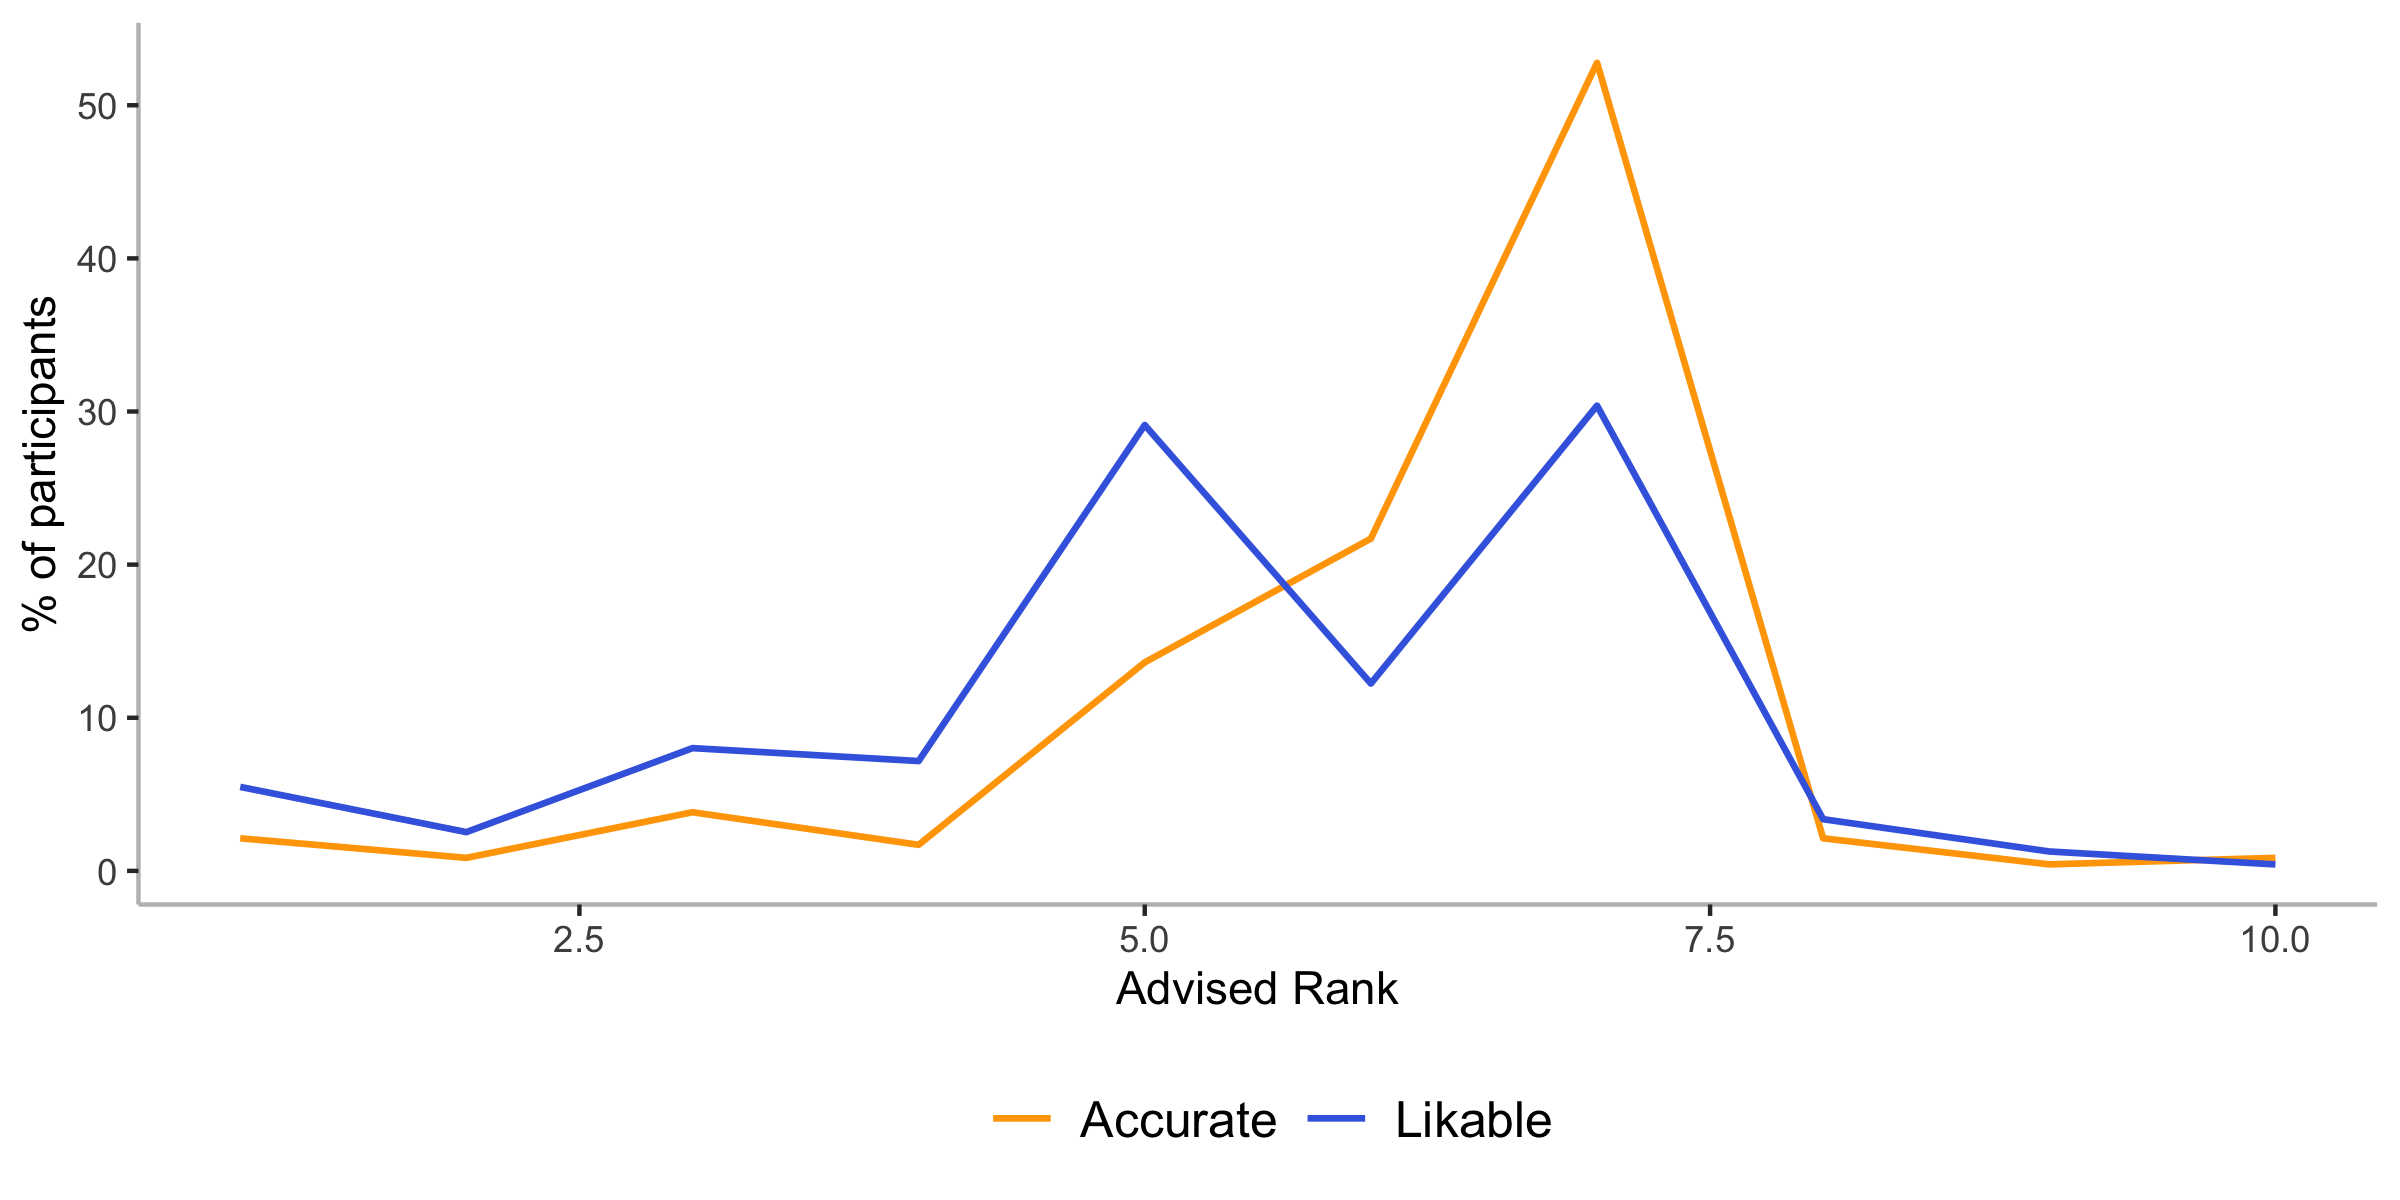
\includegraphics{Advice-Giving_files/figure-latex/study2advice-1} 

}

\caption{Advice for 7th most attractive participants}\label{fig:study2advice}
\end{figure}

First, in line with our prediction, participants advised a lower rank (that is, more attractive) in the likeability treatment than the accuracy treatment, \(M_{\text{Likable}}\) =5.38 and \(M_{\text{Accurate}}\) = 6.19, \(t(470) = 5.44\), \(p < .001\). As seen in Figure \ref{fig:study2advice}, notably, even in the accuracy treatment, participants advised a lower rank than they themselves had provided (\(t(234) = -8.82\), \(p < .001\)). This suggests that advisers inferred that advising someone that they were more attractive would make the adviser appear more likable and therefore provided advice that communicated a more favorable impression of the participants' attractiveness.

\begin{table}

\caption{\label{tab:study2regs}When individuals receive advice that implies a high level of attractiveness (lower rank), they tend to perceive the advice giver as more likable (Column 1) and warm (Column 2).}
\centering
\resizebox{\linewidth}{!}{
\begin{tabular}[t]{lcc}
\toprule
  & (1) & (2)\\
\midrule
Advised Rank & \num{-0.109}* & \num{-0.133}**\\
 & (\num{0.046}) & (\num{0.044})\\
Constant & \num{3.777}*** & \num{3.903}***\\
 & (\num{0.279}) & (\num{0.266})\\
\midrule
N & \num{146} & \num{146}\\
\bottomrule
\multicolumn{3}{l}{\rule{0pt}{1em}+ p $<$ 0.1, * p $<$ 0.05, ** p $<$ 0.01, *** p $<$ 0.001}\\
\end{tabular}}
\end{table}

\begin{figure}

{\centering 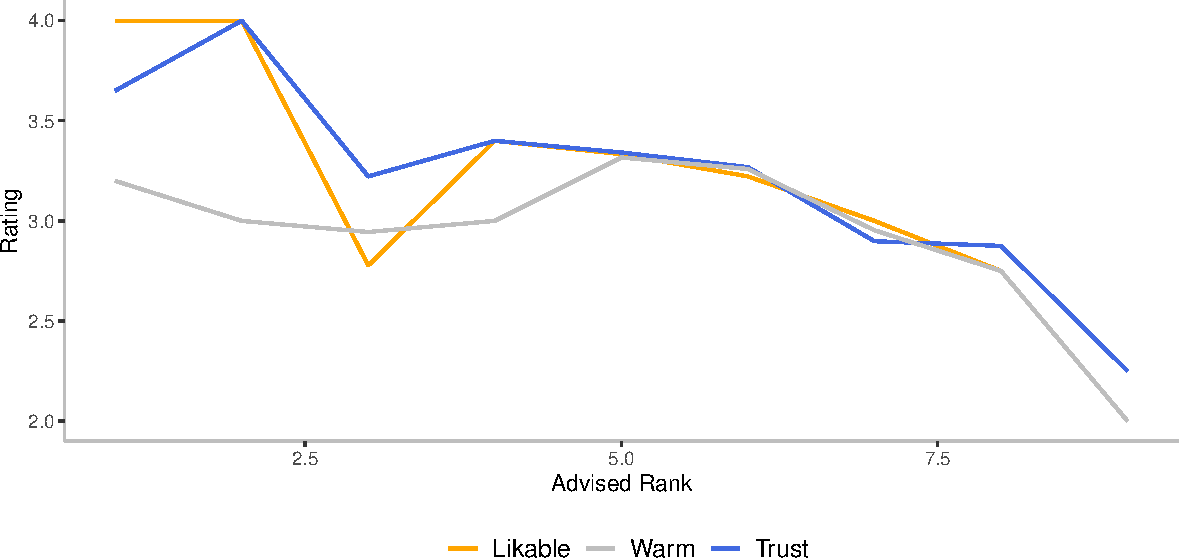
\includegraphics{Advice-Giving_files/figure-latex/study2rating-1} 

}

\caption{The evaluation of advice givers}\label{fig:study2rating}
\end{figure}

Of the 200 advisees, 73\% returned for a follow-up survey, provided their incentivized guess, and evaluated advisers on likeability and warmth. As seen in Figure \ref{fig:study2rating}, in line of our predictions, we found that advisees who suggested that the advisee was more attractive were indeed rated as more likeable (Column 1 of Table \ref{tab:study2regs} ), and warmer (Column 2 of Table \ref{tab:study2regs} ). Notably, however, we were not powered to do a comparison across the two experimental groups.


\end{document}
